\documentclass[border=4pt]{standalone}
\usepackage[T1]{fontenc}
\usepackage{helvet}
\renewcommand{\familydefault}{\sfdefault}
\usepackage{graphicx}
\usepackage{caption}
\usepackage{amsmath}
\captionsetup{font={sf,footnotesize},labelfont={sf,bf,footnotesize},justification=justified,singlelinecheck=false}
\begin{document}
\setcounter{figure}{7}
\begin{minipage}{7.20in}
\centering
\begin{figure}[htbp]
    \centering
    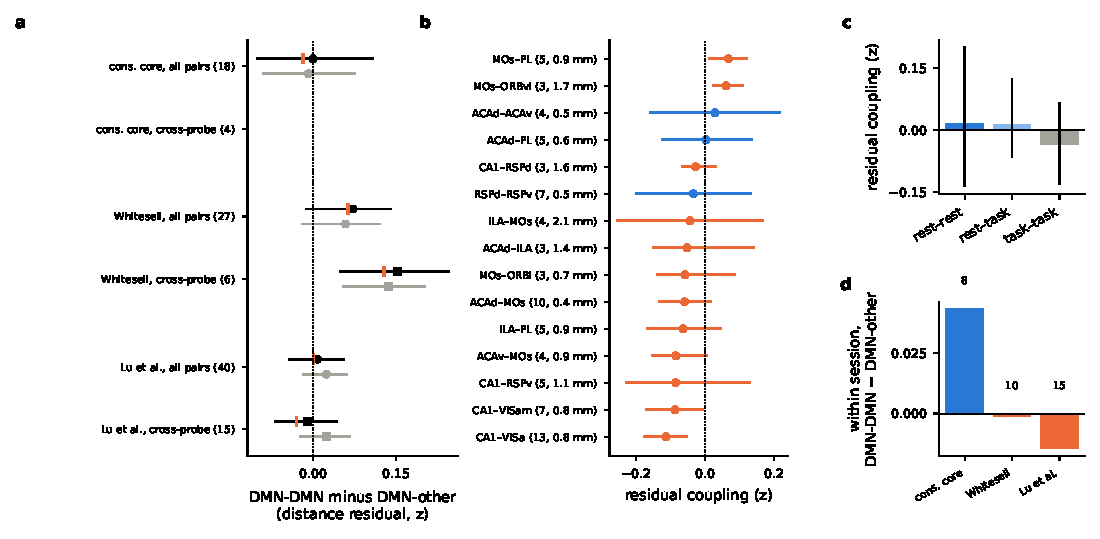
\includegraphics[width=\linewidth]{fig8_coupling_panels.pdf}
    \caption{\textbf{a} Grey-screen co-fluctuation of region signals for the conservative core (still bins only; wheel, lick and motion-energy regression), as residual from cortical and CA1 pairs at the same distance and probe relation. Differences between pair classes (cortical pairs only), 1 s (black) and 0.5 s (grey) bins, 95\% mouse-bootstrap CI (18 mice with a core--core pair). Only 4 core--core pairs come from two probes, too few to test separately. \textbf{b} Residual coupling per pair class, averaged per mouse (dots; number of mice at the bottom), black: mean and 95\% bootstrap CI. \textbf{c} Every recorded core pair: mean residual coupling over mice, with 95\% bootstrap CI where $\geq$3 mice (open markers: fewer mice). Within session, core--core minus core--other coupling is +0.04 (8 mice, Wilcoxon p = 0.64).}
    \label{fig:grey_coupling}
\end{figure}
\end{minipage}
\end{document}
